\documentclass[UTF8]{article}

\usepackage{ctex}
\usepackage{marginnote}
\usepackage{listings}
\usepackage[dvipdfm]{graphicx}
\usepackage{subfig}
\usepackage[dvipsnames]{xcolor}
\usepackage{xcolor}
%\usepackage[svgnames]{xcolor}
%\usepackage[x11names]{xcolor}
%\usepackage{xcolor}

\title{插图}
\author{Xmp}
\date{\today}
\begin{document}
\setcounter{tocdepth}{10}
\maketitle
\begin{abstract}
	\begin{quote}
		A picture says more than a thousand words.
		
		\marginnote{---Shakespeare}
		\reversemarginpar
	\end{quote}
\end{abstract}
\tableofcontents


\section{图形概览}
\subsection{图形格式}
对于示意图,我们应该首选矢量格式;包含大量自然色彩的图像 (比如照片)应该选 JPEG;人工点阵图像应该选 PNG。

\subsection{Driver的口味}
\subsubsection{dvips}
\subsubsection{pdflatex}
\subsubsection{dvipdfm(x)}
\subsubsection{xdvipdfmx}

\subsection{图形优化}
矢量图形的一个优点是可以无限缩放,而输出质量不变。图形尺寸对矢量图形而言意义不大。描述矢量图形所需数据较少,所以其文件体积一般也较小。

而点阵图形是以像素 (pixel) 为单位描述、存储的,图形尺寸越大,文件体积就越大。当然影响文件体积的还有色彩深度、压缩算法等因素。

人们一般希望用较小的文件体积获取较好的输出效果,这样就需要优
化图形尺寸和色彩。

\subsubsection{图形尺寸}
点阵图形的信息量取决于像素。图形文件的分辨率只是“建议”缺省输出尺寸,并不影响图形质量。上述操作中裁剪和改尺寸比较实用,改分辨率没有实质意义。改尺寸一般也只能从大改小。如果从小改大的话,插补出来的像素比起原装的还是要差一些。

\subsubsection{色彩深度}
我们一般也只能把图形的色深从高改低,从而减小图形文件和最终文档的体积。

\subsection{图形转换和处理}
命令行界面推荐ImageMagick,
\subsubsection{其他格式转为EPS}
ImageMagick 转换 EPS 的方法如下。如果是 BMP 文件,最好先压缩成JPEG 或 PNG,再转为 EPS,这样生成的 EPS 会比较小。我猜 EPS 的缺省压缩算法可能不如 JPEG 和 PNG。

convert fig.png eps3:fig.eps

另一种方法是用虚拟打印机生成 EPS,它的优点是可以把几乎所有文件“打印”成 EPS。推荐 Bullzip \emph{PDF Printer},它可以把各种文件打印成PS、EPS、PDF、BMP、JPEG、PCX、PNG、TIFF 等格式。用合适的软件打开原始文件,打印到 Bullzip PDF Printer。在 General 标签页把 Format 设置为 EPS,点 Save 按钮就会得到 EPS。

\section{插入图形}
\subsection{范围框}
由于历史原因,latex编译程序不能提取JPEG、PNG等点阵图形的尺寸信息,所以它在处理这些图形文件时需要范围框 (bounding box) 。pdflatex和 xelatex 的用户可以跳过此处,因为它们出现的比较晚,有机会了解这些图形格式。

\subsection{基本命令}
使用graphics和graphicx宏包,插图命令基本用法如下:
\lstset
{
numbers=left, 
numberstyle= \tiny, 
keywordstyle= \color{ blue!70},
commentstyle= \color{red!50!green!50!blue!50}, 
frame=shadowbox, % 阴影效果
rulesepcolor= \color{ red!20!green!20!blue!20} ,
escapeinside=``, % 英文分号中可写入中文
xleftmargin=2em,xrightmargin=2em, aboveskip=1em,
framexleftmargin=2em
}
\begin{lstlisting}
	\usepackage[dvipdfm]{graphicx}
	\includegraphics[bb=0 0 300 200]{fig.png}
\end{lstlisting}

\subsection{图形操作}
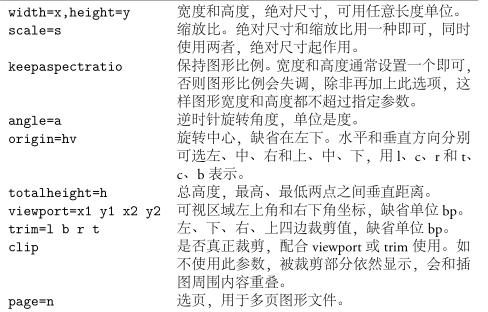
\includegraphics[scale=1.0]{GraphicalOperation.png}
\\
\\

图形缩放
\\
\\

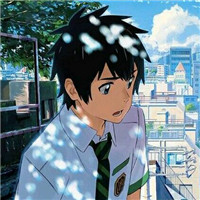
\includegraphics[width=60pt]{test.jpg}
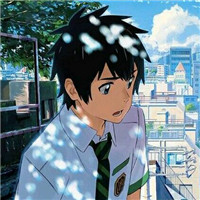
\includegraphics[width=80pt]{test.jpg}
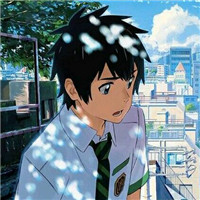
\includegraphics[width=80pt,height=100pt]{test.jpg}
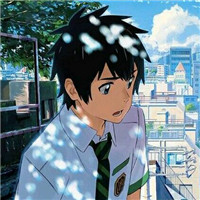
\includegraphics[width=80pt,height=100pt,keepaspectratio]{test.jpg}
\\
\\

图形旋转


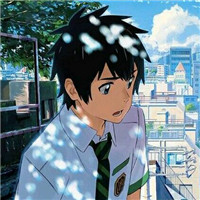
\includegraphics[width=60pt,angle=90]{test.jpg}
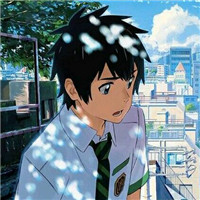
\includegraphics[width=60pt,angle=180]{test.jpg}
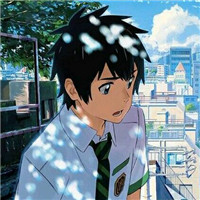
\includegraphics[width=60pt,angle=270]{test.jpg}\\
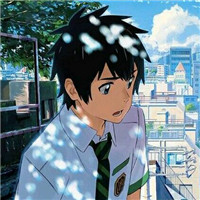
\includegraphics[width=60pt,angle=90,origin=c]{test.jpg}
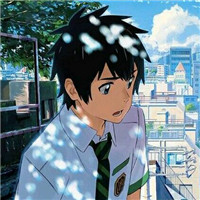
\includegraphics[width=60pt,angle=180,origin=c]{test.jpg}
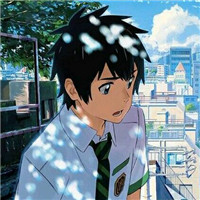
\includegraphics[width=60pt,angle=270,origin=c]{test.jpg}\\

\subsection{文件名和路径}
若想省略文件后缀或路径名,可以使用下面的命令。其中第一行指定后缀列表让编译程序自行查找;第二行指出未知后缀的都是EPS;后三行设置缺省搜索路径,分别使用了绝对路径、相对路径、多个路径。注意文件名和路径名都不能有空格;路径名分隔符最好用正斜杠/,这样可以在多种操作系统上通用;路径名要用/结尾。

%前面设置了代码的显示格式\lsset{},故此处直接使用
\begin{lstlisting}
\DeclareGraphicsExtensions{.eps,.mps,.pdf
	  ,.jpg,.png}
\DeclareGraphicsRule{*}{eps}{*}{}
\graphicspath{{c:/secret-garden/}}
\graphicspath{{./img/}}
\graphicspath{{one-little/}{two-little/}{three
	 -little-indians/}}
\end{lstlisting}

\subsection{figure环境}
htbp选项用来指定插图的理想位置,这几个字母分别代表here,top,bottom,float page,也就是就这里、页顶、页尾、浮动页(专门放浮动环境的单独页面)。

我们可以使用这几个字母的任意组合,四个母都写上表示放哪里都无所谓;一般不推荐单独使用h,因为\LaTeX 自以为它的排版算法是最完美的,不愿意被束缚手脚。\textbackslash centering用来使插图居中;\textbackslash caption命令设置插图标题,\LaTeX 会自动给浮动环境的标题加上编号。注意\textbackslash label应该放在标题之后,否则引用时指向的是前一个结构对象。
\begin{figure}[htbp]
\centering
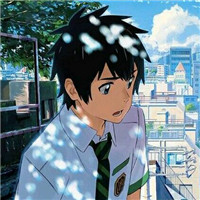
\includegraphics[width=80pt]{test.jpg}
\caption{测试图片}
\label{fig:myphoto}
\end{figure}

\subsection{插入多幅图形}
\subsubsection{并排摆放,共享标题}
\begin{figure}[htbp]
\centering
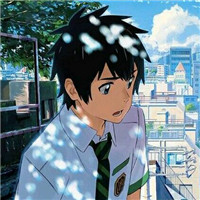
\includegraphics[width=60pt]{test.jpg}
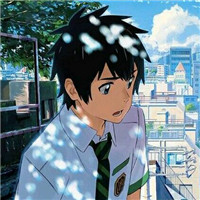
\includegraphics[width=60pt]{test.jpg}
\caption{并排摆放,共享标题}
\end{figure}

\subsubsection{并排摆放,各有标题}
\begin{figure}[htbp]
\centering
\begin{minipage}{80pt}
	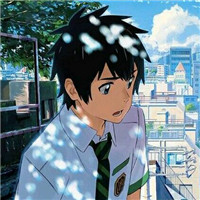
\includegraphics[width=80pt]{test.jpg}
	\caption{第一张图}
\end{minipage}
\hspace{10pt}
\begin{minipage}{80pt}
	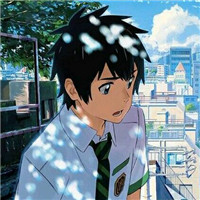
\includegraphics[width=80pt]{test.jpg}
	\caption{第二张图}
\end{minipage}
\end{figure}

\subsubsection{并排摆放,共享标题,各有子标题}%使用subfig宏包
\begin{figure}[htbp]
\centering
\subfloat[左边图片]{
	\label{fig:subfig_a}
	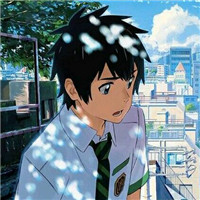
\includegraphics[width=80pt]{test.jpg}
}
\hspace{10pt}
\subfloat[右边图片]{
	\label{fig:subfig_b}
	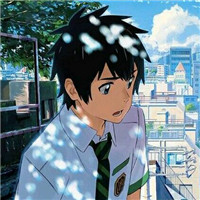
\includegraphics[width=80pt]{test.jpg}
}
\caption{共享标题}
\end{figure}

\subsubsection{改进的子图方法}
\textbackslash subfloat命令缺少宽度参数,而子标题最多只能和子图一样宽,太长的话会出现折行。为了避免子标题折行,我们可以在\textbackslash subfloat里再嵌套个minipage,因为后者是有宽度的。
\begin{figure}[htbp]
	\centering
	\subfloat[左边图片]{
		\label{fig:improved_subfig_a}
		\begin{minipage}[t]{80pt}
		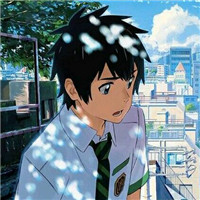
\includegraphics[width=80pt]{test.jpg}
		\centering
		\end{minipage}
		
	}
	\hspace{10pt}
	\subfloat[右边图片]{
		\label{figimproved_:subfig_b}
		\begin{minipage}[t]{80pt}
			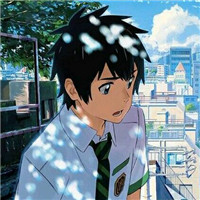
\includegraphics[width=80pt]{test.jpg}
			\centering
		\end{minipage}
	}
	\caption{改进的共享标题}
\end{figure}

\section{矢量绘图}
\subsection{色彩模型}
\subsubsection{预定义和自定义颜色}
xcolor宏包中预定义的颜色有:19种基本颜色,68种dvips颜色,151种SVG颜色,317种Unix/X11颜色。如要使用后三类颜色,引用宏包时需加相应预定义颜色集合选项:
\begin{lstlisting}
\usepackage[dvipsnames]{xcolor}
\usepackage[svgnames]{xcolor}
\usepackage[x11names]{xcolor}
\end{lstlisting}
如果这几百种预定义颜色还不能满足需要,可以使用\textbackslash definecolor命令自定义更多颜色。语法: 
\begin{lstlisting}
\definecolor{名称}{模式}{参数}
例如:
\definecolor{myred}{RGB}{255,0,0}
\definecolor{mygreen}{HTML}{00FF00}
\definecolor{myblue}{rgb}{0,0,1}
\end{lstlisting}

\subsubsection{彩色文字}
设置文字的颜色可以使用\textbackslash textcolor命令,下面例子中代码第2–4行和第5–7行输出效果相同。后三行的方法又称为抛弃型颜色定义法,因为只能用一次;事先定义了名字的话还可以重用。
\begin{lstlisting}
\textcolor{名称}|[模式]{代码}{文字}	
\end{lstlisting}
例如:
\textcolor{red}{红}
\textcolor{green}{绿}
\textcolor{blue}{蓝}
\textcolor[RGB]{255,0,0}{红}
\textcolor[HTML]{00FF00}{绿}
\textcolor[rgb]{0,0,1}{蓝}

\subsubsection{彩色盒子}
语法和彩色文字差不多,\textbackslash colorbox命令生成有彩色背景的盒子,\textbackslash fcolorbox给彩色盒子加了边框,第一个参数是边框的颜色。\\
\colorbox{Lavender}{text}
\colorbox{SkyBlue}{text}
\fcolorbox{SkyBlue}{Lavender}{text}
\fcolorbox{Lavender}{SkyBlue}{text}

\subsection{绘图工具概览}
目前不太清楚,对绘图这方面我也不指望使用\LaTeX 绘制,使用Visio或者别的绘制效率更高,之后在插入文档之中。

就目前了解的情况,感觉TiKZ比较高级。

\end{document}